% =============================================================================

\section{Intro}

% =============================================================================

\SlideTextA{Informações Gerais e Título}{

    \textbf{Autor:} Wesley Rodrigues da Silva

    \bigskip

    \textbf{Título:} Um Framework de Segurança de Dados na Nuvem para Indústria
    Financeira.
}

% =============================================================================

\section{Problema}

% =============================================================================

\SlideTextA{Problema - Contexto}{

    \ABNTfigure
    {Captura de tela mostrando novos países com CBDCs.}
    {Adaptado de Atlantic Council \citeyear{CBDCTracker2022}.}
    {figures/WORLD.png}
    {width=0.7\textwidth}
    {fig:CBDCTracker2022}
}

% =============================================================================

\SlideTextA{Problema - Contexto}{

    \ABNTfigure
    {BACEN mostrando a arquitetura do Real Digital.}
    {\textcite{BACEN2023}.}
    {figures/BACEN.png}
    {width=0.6\textwidth}
    {fig:BACEN2023}

}

% =============================================================================

\SlideTextA{Problema - Contexto}{

    \ABNTfigure
    {HTTP vs HTTPS.}
    {\textcite{HTTPS2023}.}
    {figures/HTTPS.png}
    {width=0.4\textwidth}
    {fig:HTTPS2023}

}

% =============================================================================

\SlideTextA{Problema - Contexto}{

    \ABNTfigure
    {Chaves públicas e privadas.}
    {\textcite{ASYMMETRIC2023}.}
    {figures/ASYMMETRIC.png}
    {width=0.7\textwidth}
    {fig:ASYMMETRIC2023}

}

% =============================================================================

\SlideTextA{Problema - Contexto}{

    \ABNTfigure
    {Dados criptografados em repouso e em trânsito.}
    {\textcite{SALESFORCE_REST_TRANSIT_2023}.}
    {figures/REST_TRANSIT.png}
    {width=0.5\textwidth}
    {fig:REST_TRANSIT}

}

% =============================================================================

\SlideTextA{Problema - Contexto}{

    \ABNTfigure
    {Dados criptografados em repouso, em trânsito e em uso.}
    {\textcite{MICROSOFT_REST_TRANSIT_USE_2023}.}
    {figures/REST_TRANSIT_USE.png}
    {width=0.6\textwidth}
    {fig:REST_TRANSIT_USE}

}

% =============================================================================

\SlideTextA{Problema - Geral}{

    \ABNTfigure
    {Principais vulnerabilidades em aplicações web.}
    {\textcite{OWASP_TOP10_2021}.}
    {figures/TOP10.png}
    {width=0.7\textwidth}
    {fig:OWASP_TOP10_2021}

}

% =============================================================================

\SlideTextA{Problema - Geral}{

    \ABNTfigure
    {Perspectivas em Cybersecurity.}
    {\textcite{PERSPECTIVES2023}.}
    {figures/PERSPECTIVES.png}
    {width=0.3\textwidth}
    {fig:PERSPECTIVES2023}

}

% =============================================================================

\SlideTextA{Problema - Geral}{

    \ABNTfigure
    {Ameaças emergentes em cybersecurity.}
    {\textcite{ENISA2023}.}
    {figures/ENISA.png}
    {width=0.6\textwidth}
    {fig:ENISA2023}

}

% =============================================================================

\SlideTextA{Problema - Geral}{

    \Large
    \begin{center}

        Os paradigmas de segurança evoluíram na última década, estamos perto de dois pontos de virada: na \textbf{economia} e na \textbf{tecnologia criptográfica}.

        Soluções com defesa em múltiplas camadas são necessárias.

        \bigskip\bigskip

        Bibliografia utilizada no contexto e levantamento dos problemas de pesquisa:
        \textcite{barros_silva_2023, boido_aliano_2023, wenhua2023, IBM_quantum_2023, runge_2022, NIST_present_2022, xu2023}

    \end{center}

}

% =============================================================================

\SlideTextA{Problema - Específico}{

    \ABNTfigure
    {O processo de privacidade de dados tem múltiplos pontos de atenção.}
    {Autor (2023).}
    {figures/MODEL6.png}
    {width=0.3\textwidth}
    {fig:MODEL6}

}

% =============================================================================

\SlideTextA{Problema - Falta Resolver}{

    \LARGE
    \begin{center}

        Falta um modelo que demonstre o papel das seis camadas aplicadas a uma mesma carga de trabalho, e que ajude no planejamento e na avaliação das práticas de criptografia de dados.

    \end{center}

}

% =============================================================================

\section{Critérios PICO}

% =============================================================================

\SlideTextA{Critério PICO e Pergunta}{

    \textbf{(P):} Arquitetos de soluções que utilizam plataformas de nuvem.\\
    \textbf{(I):} Desenvolvimento e uso de um framework baseado em uma métrica de maturidade e definição de práticas de criptografia de dados na avaliação das arquiteturas de nuvem.\\
    \textbf{(C):} levantamento exploratório de evidências na literatura científica e/ou cinzenta.\\
    \textbf{(O):} um framework que auxilia os arquitetos na avaliação da maturidade e nas boas práticas modernas de criptografia de dados.\\

    \bigskip

    A seguinte questão de pesquisa da revisão foi elaborada por meio dos critérios
    PICO:

    \bigskip

    \textbf{
        Como desenvolver um framework de melhores práticas modernas de criptografia de dados e avaliação com score de soluções em nuvem que apoie os arquitetos de soluções que utilizam essas plataformas?
    }

}

% =============================================================================

\section{Palavras Chave e Pesquisa}

% =============================================================================

\SlideTextA{Palavras Chave (pt e en)}{

    % \ABNTboard{caption}{reference}{label}{tabular}
    \ABNTboard
    {Palavras em português e inglês}
    {Elaborado pelo autor.}
    {board:keywords}
    {
        \begin{tabular}{|l|l|}
            \hline
            \textbf{português}              & \textbf{inglês}           \\ \hline
            criptografia de dados           & data encryption           \\ \hline
            computação na nuvem             & cloud computing           \\ \hline
            avaliação de segurança          & security assessment       \\ \hline
            criptografia pós-quântica       & post-quantum cryptography \\ \hline
            módulo de segurança em hardware & hardware security module  \\ \hline
            computação confidencial         & confidential computing    \\ \hline
            protocolos de conhecimento zero & zero knowledge protocols  \\ \hline
        \end{tabular}
    }

}

% =============================================================================

\SlideTextA{String de Pesquisa}{

    As buscas em português no Web of Science não foram promissoras.
    A string de pesquisa foi montada em inglês usando o seguinte racional:

    \bigskip

    \textbf{\Large{What?}}

    \begin{itemize}
        \item privacy
        \item data encryption
        \item security assessment
    \end{itemize}

}

% =============================================================================

\SlideTextA{String de Pesquisa}{

    As buscas em português no Web of Science não foram promissoras.
    A string de pesquisa foi montada em inglês usando o seguinte racional:

    \bigskip\bigskip

    \textbf{\Large{Where?}}

    \begin{itemize}
        \item cloud computing
        \item AWS
        \item AZURE
        \item GCP
    \end{itemize}

}

% =============================================================================

\SlideTextA{String de Pesquisa}{

    As buscas em português no Web of Science não foram promissoras.
    A string de pesquisa foi montada em inglês usando o seguinte racional:

    \bigskip\bigskip

    \textbf{\Large{How?}}

    \begin{multicols}{2}
        \begin{itemize}
            \item post-quantum cryptography
            \item hardware security module
            \item confidential computing
            \item zero knowledge protocols
                  \columnbreak
            \item HSM
            \item SGX
            \item SEV-SNP
        \end{itemize}
    \end{multicols}

}

% =============================================================================

\SlideTextA{String de Pesquisa}{

    A string final ficou definida da seguinte forma:

    \bigskip

    {
        \large
        {\setlength{\parindent}{0cm}
            \ttfamily
            TS=("privacy" OR "data encryption" OR "security assessment") AND\par
            TS=("cloud computing" OR "AWS" OR "AZURE" OR "GCP") AND\par
            TS=("post-quantum cryptography" OR "hardware security module" OR\par
            "confidential computing" OR "zero knowledge protocols" OR\par
            "HSM" OR "SGX" OR "SEV-SNP")\par
        }
    }

    \bigskip

    Foi aplicado um critério de restrição temporal permitindo artigos dos últimos 5 anos.
}

% =============================================================================

\SlideTextA{Web of Science -- Busca Avançada}{

    \ABNTfigure
    {Tela de busca do Web of Science.}
    {Autor (2023).}
    {figures/SEARCH_WOS.png}
    {width=0.7\textwidth}
    {fig:SEARCH_WOS}

}

% =============================================================================

\section{VosViewer - Palavras Chave}

% =============================================================================

\SlideTextA{Correlação de Palavras Chave -- VosViewer}{

    \begin{figure}[ht]
        \centering
        \caption{Parâmetros para obter as redes de palavras chaves no VosViewer.}
        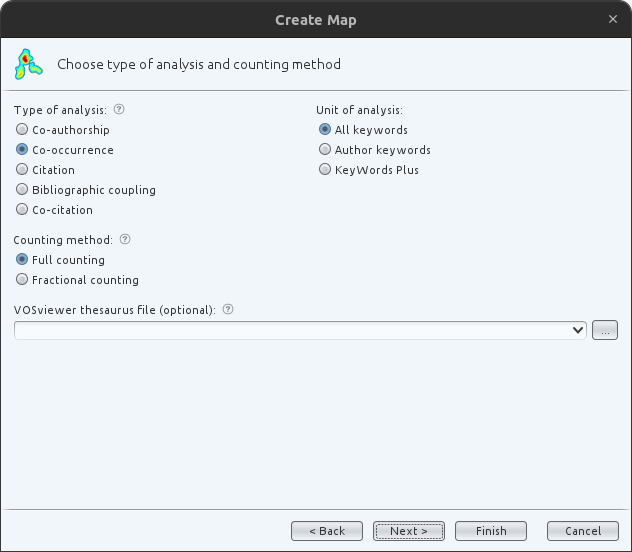
\includegraphics[width=0.4\textwidth]{figures/bibliometry/VOS_KEYWORDSa.png}
        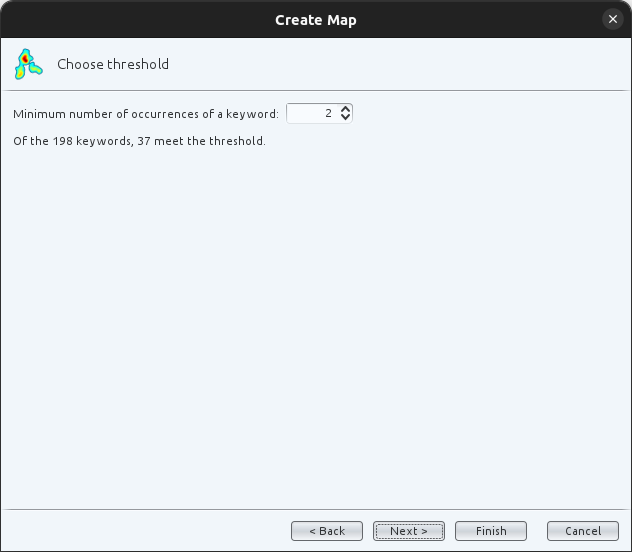
\includegraphics[width=0.4\textwidth]{figures/bibliometry/VOS_KEYWORDSb.png}
        \caption*{\textbf{Fonte:} Autor (2023).}
        \label{fig:VOS_KEYWORDSab}
    \end{figure}

}

% =============================================================================

\SlideTextA{Correlação de Palavras Chave -- VosViewer}{

    \begin{figure}[ht]
        \centering
        \caption{Principais palavras chaves e suas redes de conexões.}
        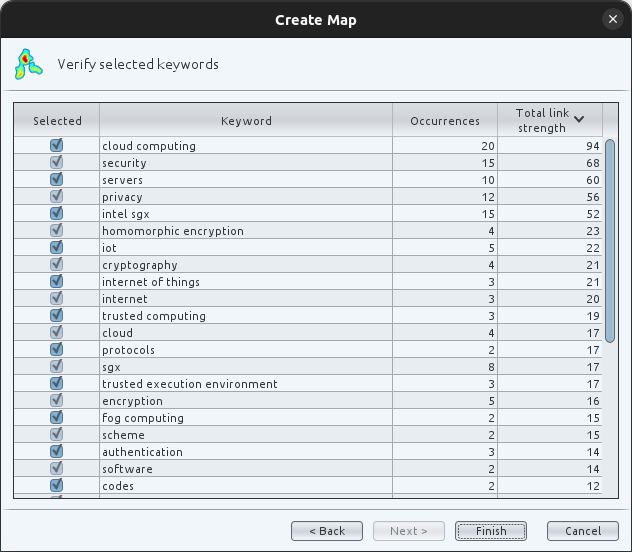
\includegraphics[width=0.4\textwidth]{figures/bibliometry/VOS_KEYWORDSc.png}
        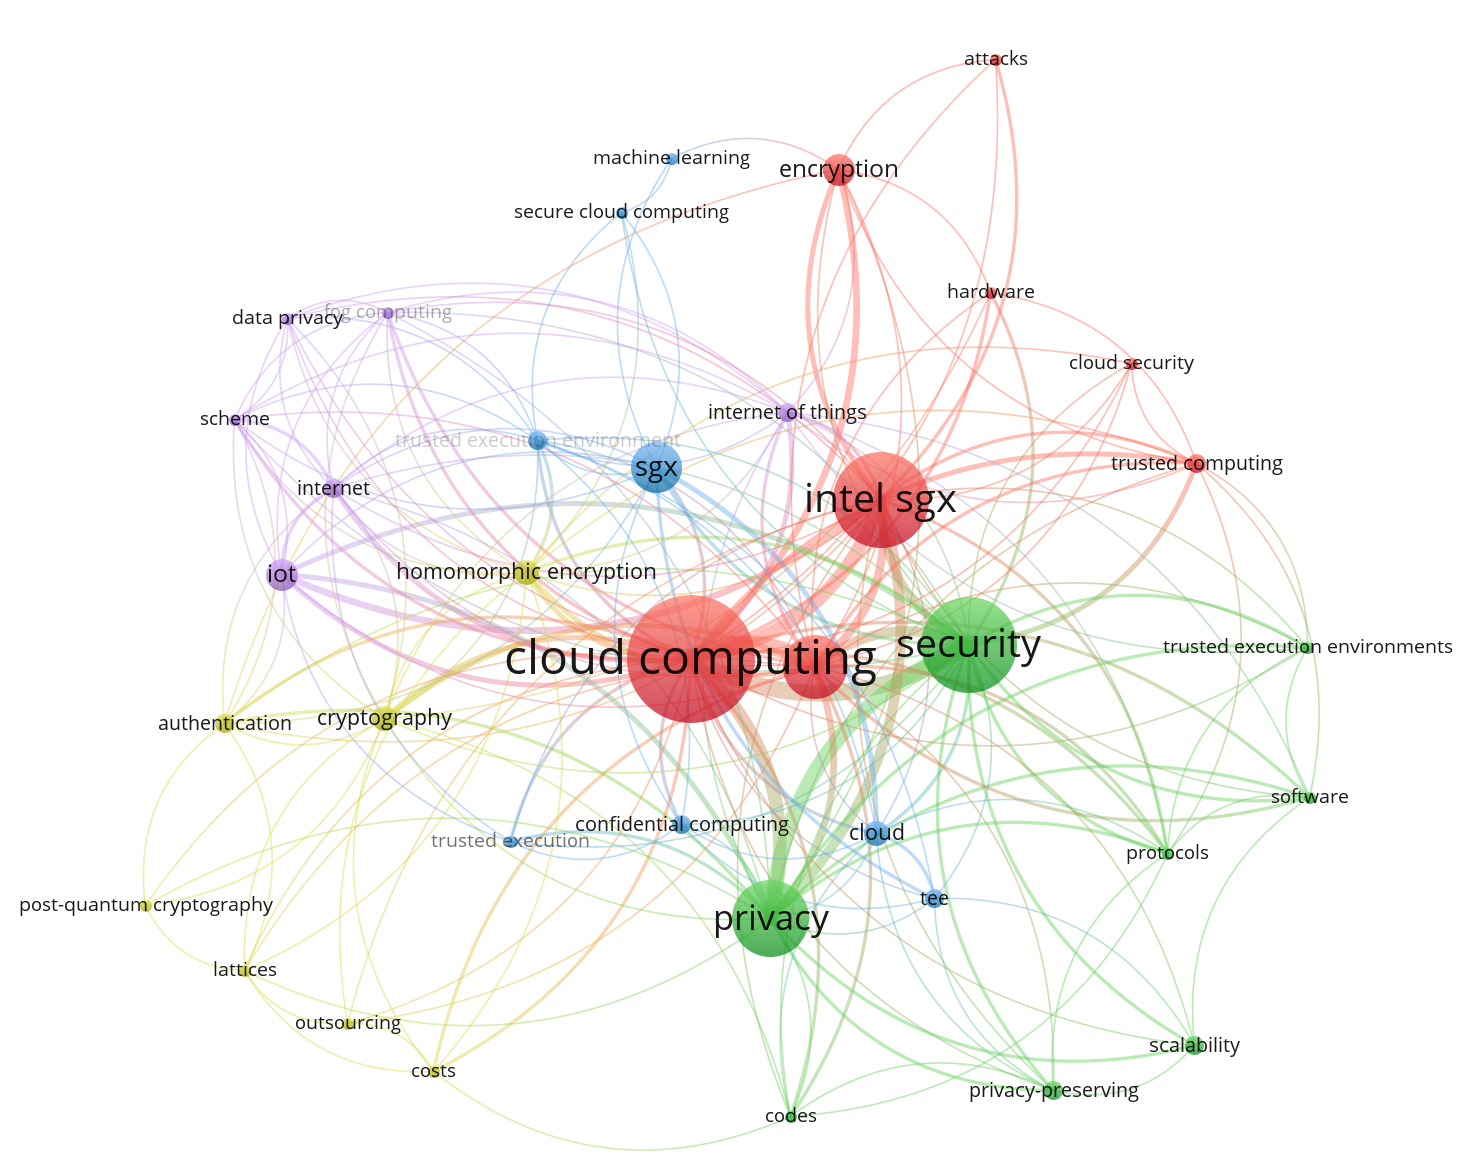
\includegraphics[width=0.4\textwidth]{figures/bibliometry/VOS_KEYWORDSd.png}
        \caption*{\textbf{Fonte:} Autor (2023).}
        \label{fig:VOS_KEYWORDScd}
    \end{figure}

}

% =============================================================================

\SlideTextA{Correlação de Palavras Chave -- VosViewer}{

    \begin{center}
        O gráfico de rede de palavras do VosViewer mostra que há grupos que não estão diretamente nos termos originais, mas que podem ser adicionados na literatura principal ou complementar.

        \bigskip

        Por exemplo, as \textbf{lattices}, que são famílias de algoritmos resistentes aos ataques quânticos, a \textbf{criptografia homomórfica}, que é uma técnica usada em computação confidencial, e os termos \textbf{fog computing} e \textbf{IoT}, que tem relação direta com a conexão entre o mundo físico e a nuvem.

    \end{center}

}

% =============================================================================

\section{Objetivos e Métodos}

% =============================================================================

\SlideTextA{Hipóteses e Proposições}{

    A hipótese levantada neste trabalho é que com um estudo da Revisão Sistemática da Literatura somado ao estudo de caso de como os três maiores provedores de nuvem atualmente (Amazon, Google e Microsoft) recomendam o uso dos serviços de proteção de dados, é possível criar um framework que apoie os arquitetos de sistemas que utilizam a nuvem na avaliação (incluindo um score de maturidade) e planejamento de seus sistemas para utilizar as práticas recentes de criptografia de dados.

}

% =============================================================================

\SlideTextA{Premissas}{

    O estudo tem como objeto de verificação soluções de Sistemas de Informação que utilizam provedores de nuvem pública, focando em Amazon Web Services, Microsoft Azure e Google Cloud Platform, que juntos têm mais de 65\% do mercado.

}

% =============================================================================

\SlideTextA{Objetivos}{

    \begin{itemize}
        \item Realizar uma RSL sobre as práticas de criptografia de dados.
        \item Realizar estudos de casos múltiplos sobre as práticas de criptografia de dados.
        \item Criar um modelo de avaliação de maturidade nos aspectos de práticas de criptografia de dados.
        \item Criar um framework que apoie os arquitetos no planejamento de práticas modernas de criptografia das camadas de segurança de dados.
    \end{itemize}

}

% =============================================================================

\SlideTextA{Contribuições Esperadas}{

    \textbf{Para a academia:} O presente trabalho entrega para a academia um compêndio com os mais recentes avanços na área da criptografia aplicada à proteção dos dados pessoais, convidando novos pesquisadores para avançar os estudos deste ramo.

    \bigskip

    \textbf{Para a indústria:} O framework pode ser utilizado de forma prática por arquitetos de software que planejam soluções que utilizam a nuvem.

}

% =============================================================================

\SlideTextA{Metodologia de Pesquisa}{

    \ABNTfigure
    {A metodologia seguida será uma RSL somada a um estudo de caso.}
    {Autor (2023).}
    {figures/METODOLOGIA.png}
    {width=0.6\textwidth}
    {fig:METODOLOGIA}

}

% =============================================================================

\section{VosViewer - Citações}

% =============================================================================

\SlideTextA{Citações por Autores -- VosViewer}{

    \begin{figure}[ht]
        \centering
        \caption{Parâmetros para obter as redes de citações por autores no VosViewer.}
        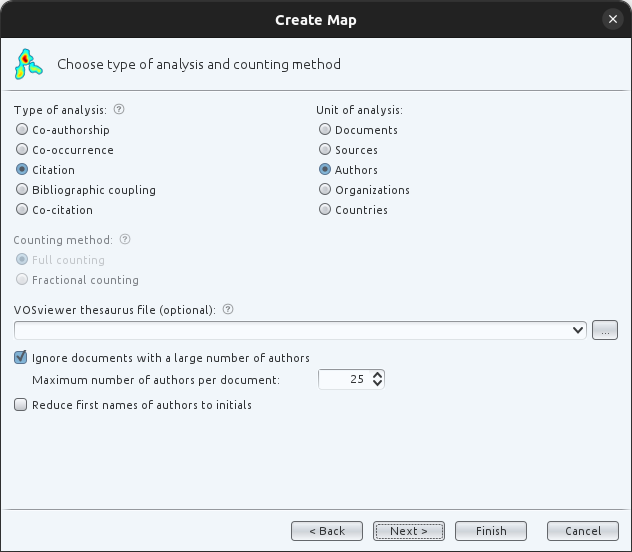
\includegraphics[width=0.4\textwidth]{figures/bibliometry/CITEa.png}
        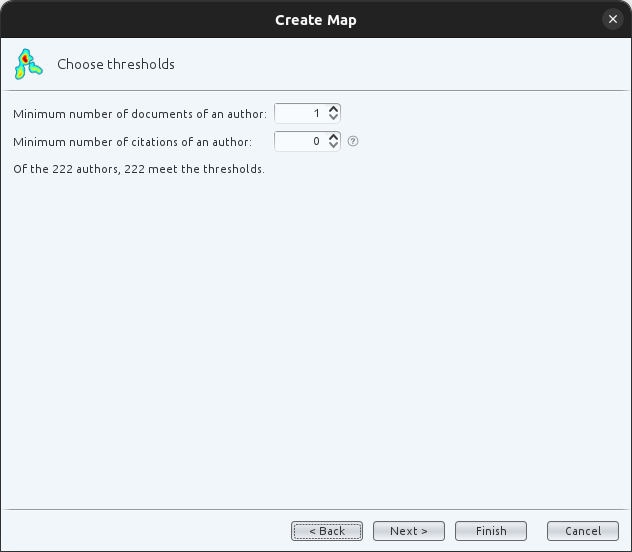
\includegraphics[width=0.4\textwidth]{figures/bibliometry/CITEb.png}
        \caption*{\textbf{Fonte:} Autor (2023).}
        \label{fig:VOS_CITEab}
    \end{figure}

}

% =============================================================================

\SlideTextA{Citações por Autores -- VosViewer}{

    \begin{figure}[ht]
        \centering
        \caption{Ordenados por força do link.}
        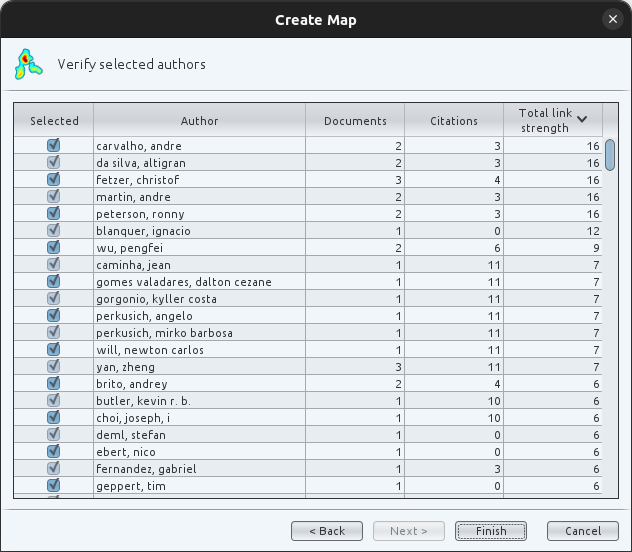
\includegraphics[width=0.35\textwidth]{figures/bibliometry/CITEc.png}
        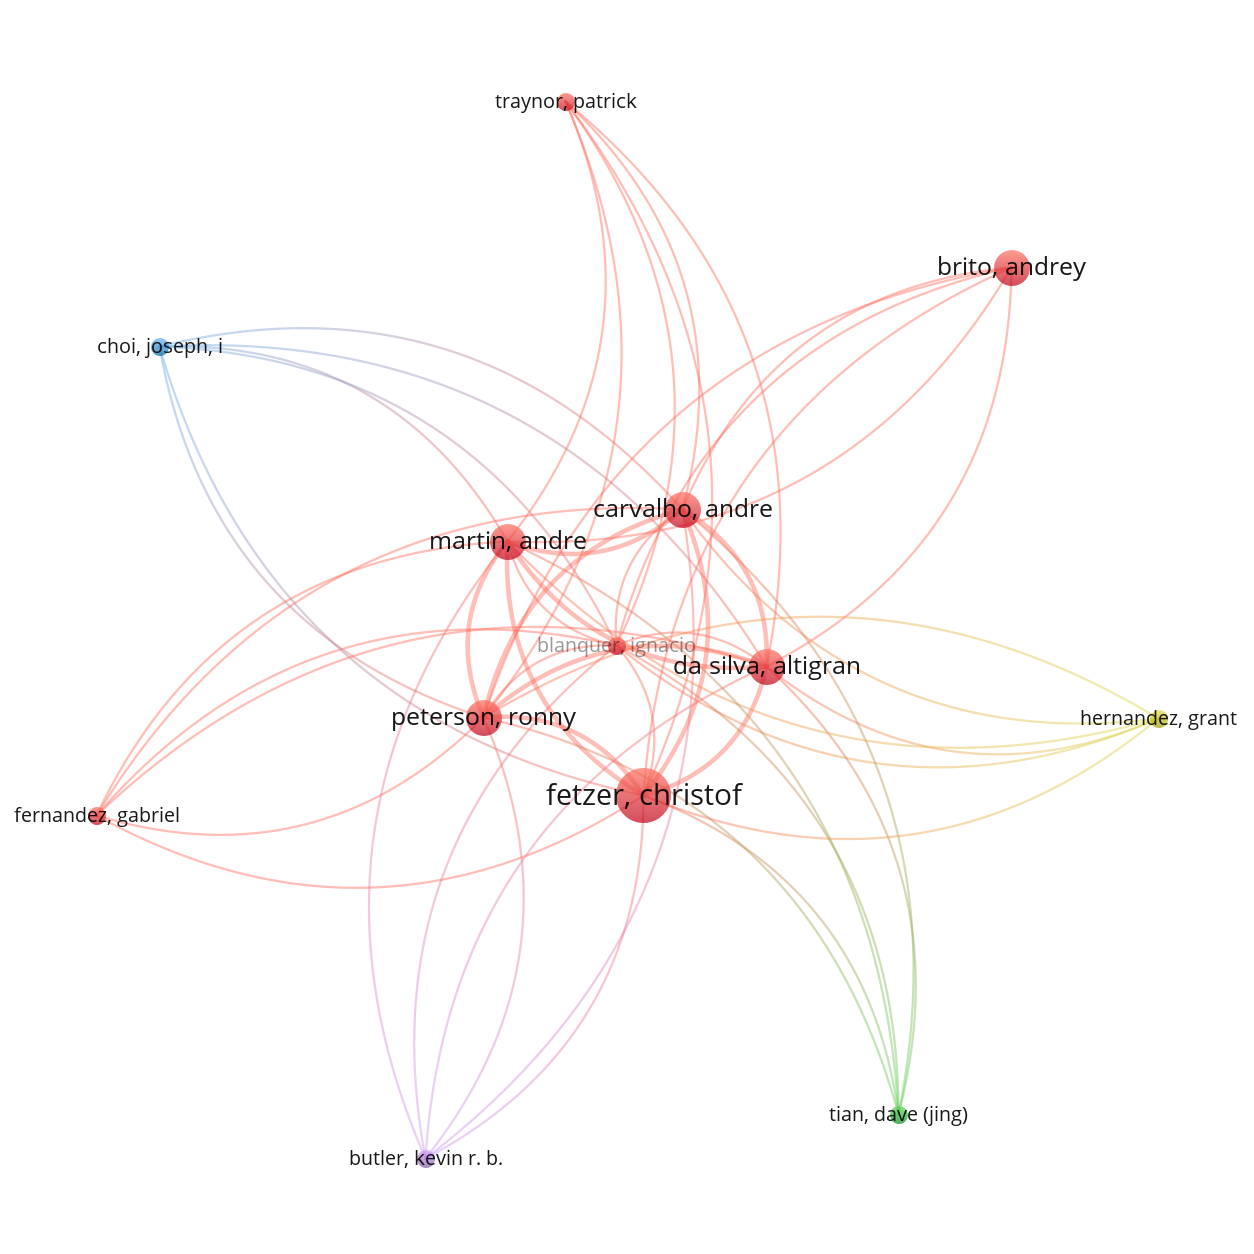
\includegraphics[width=0.35\textwidth]{figures/bibliometry/CITEe.png}
        \caption*{\textbf{Fonte:} Autor (2023).}
        \label{fig:VOS_CITEce}
    \end{figure}

}

% =============================================================================

\SlideTextA{Citações por Autores -- VosViewer}{

    \begin{figure}[ht]
        \centering
        \caption{Ordenados por quantidade de citações.}
        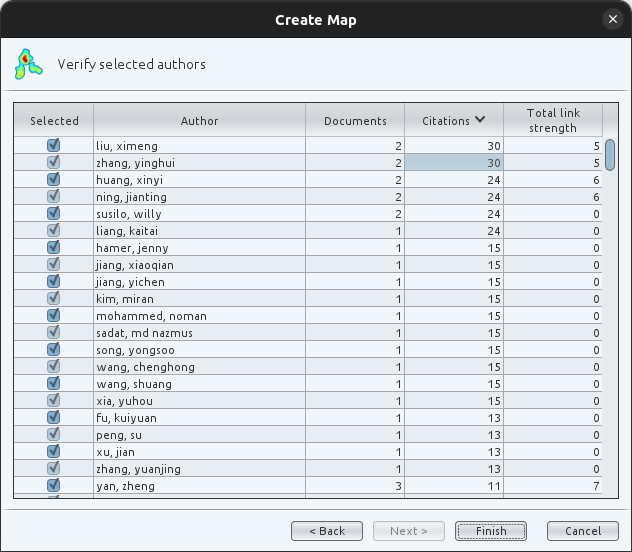
\includegraphics[width=0.35\textwidth]{figures/bibliometry/CITEd.png}
        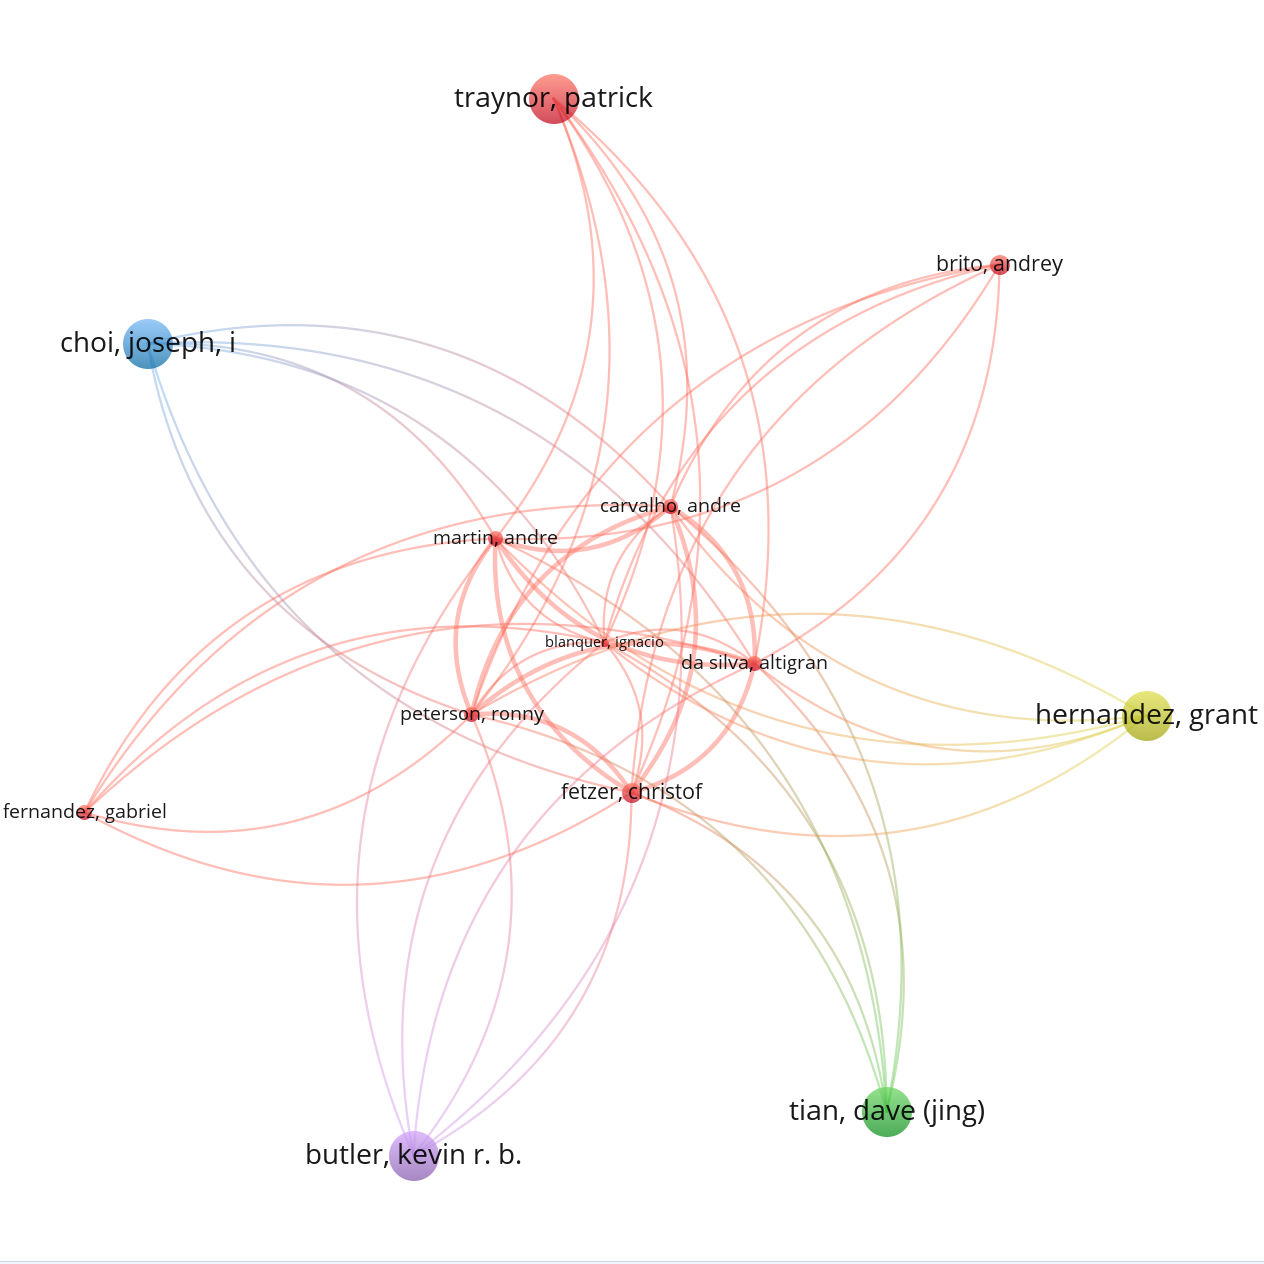
\includegraphics[width=0.35\textwidth]{figures/bibliometry/CITEf.png}
        \caption*{\textbf{Fonte:} Autor (2023).}
        \label{fig:VOS_CITEdf}
    \end{figure}

}

% =============================================================================

\SlideTextA{Artigos Mais Citados -- VosViewer}{

    Os 3 artigos lidos (abstract e keywords) são relevantes para o trabalho:

    \begin{itemize}
        \item \textcite{VOS_SGX}: Este artigo contribui com o tópico de proteção dos dados, isolando o ambiente em nuvem de forma que o operador da nuvem não tenha acesso aos dados do cliente, mesmo controlando o virtualizador e o hardware.
        \item \textcite{VOS_END2END}: Apesar de usar a nuvem, os dados normalmente são gerados fora da nuvem. Este artigo trata do processo de proteção de ponta a ponta.
        \item \textcite{VOS_VALLUM}: Tópicos como criptografia homomórfica e suportada por hardware são abordados neste artigo que foca em privacidade de dados.
    \end{itemize}


}

% =============================================================================
